\documentclass{article}

% content/resources/templates/preamble.tex
\usepackage[margin=0.6in]{geometry}
\author{Milav Dabgar}
\usepackage{amsmath,amssymb,amsthm}
\usepackage{booktabs}
\usepackage{multirow}
\usepackage{xcolor}
\usepackage{tcolorbox}
\tcbuselibrary{breakable,skins}
\usepackage[colorlinks=true,linkcolor=blue]{hyperref}
\usepackage{titlesec}
\usepackage{enumitem}
\usepackage{tikz}
\usepackage{pgfplots}
\usepackage{circuitikz}
\usepackage[version=4]{mhchem}
\usepackage{longtable}
\usepackage{array}
\usepackage{float}
\usepackage{caption}
\usepackage{listings}

\lstset{
  basicstyle=\small\ttfamily,
  breaklines=true,
  breakatwhitespace=false,
  postbreak=\mbox{\textcolor{red}{$\hookrightarrow$}\space},
  float=false,
  numbers=left,
  numberstyle=\tiny\color{gray},
  numbersep=10pt,
  xleftmargin=2em,
  keywordstyle=\color{blue},
  commentstyle=\color{green!60!black},
  stringstyle=\color{purple},
  backgroundcolor=\color{gray!5},
  showstringspaces=false,
  tabsize=2,
  captionpos=b,
  keepspaces=true,
  columns=flexible
}

\pgfplotsset{compat=1.18}
\usetikzlibrary{shapes,arrows,positioning,calc,patterns,decorations.pathmorphing,decorations.markings,arrows.meta}

% Color scheme
\definecolor{headcolor}{RGB}{0,102,204}
\definecolor{keycolor}{RGB}{220,20,60}
\definecolor{solutioncolor}{RGB}{34,139,34}
\definecolor{mnemoniccolor}{RGB}{148,0,211}
\definecolor{codecolor}{RGB}{0,0,100}

% Spacing
\setlength{\parskip}{3pt}
\setlist[itemize]{nosep}
\setlist[enumerate]{nosep}

% Title formatting
\titleformat{\section}{\Large\bfseries\color{headcolor}}{\thesection}{1em}{}
\titleformat{\subsection}{\large\bfseries\color{headcolor}}{\thesubsection}{1em}{}

% Pandoc tightlist compatibility
\providecommand{\tightlist}{%
  \setlength{\itemsep}{0pt}\setlength{\parskip}{0pt}}

% Pandoc longtable compatibility
\newcounter{none}
\def\thenone{}


% content/resources/templates/english-boxes.tex

% Custom environments
\newtcolorbox{solutionbox}{
 breakable,
 enhanced,
 colback=solutioncolor!5!white,
 colframe=solutioncolor!75!black,
 fonttitle=\bfseries,
 title=Solution
}

\newtcolorbox{solutionboxnobreak}{
 colback=solutioncolor!5!white,
 colframe=solutioncolor!75!black,
 fonttitle=\bfseries,
 title=Solution
}

\newtcolorbox{keyformula}{
 breakable,
 enhanced,
 colback=keycolor!5!white,
 colframe=keycolor!75!black,
 fonttitle=\bfseries,
 title=Key Formula
}

\newtcolorbox{mnemonicboxenv}{
 breakable,
 enhanced,
 colback=mnemoniccolor!5!white,
 colframe=mnemoniccolor!75!black,
 fonttitle=\bfseries,
 title=Mnemonic
}

\newcommand{\mnemonicbox}[1]{%
  \begin{mnemonicboxenv}
    #1
  \end{mnemonicboxenv}
}


% Custom commands for GTU solutions
% This file defines semantic commands for consistent formatting

% Question command with automatic formatting
\newcommand{\question}[2]{%
  \section*{Question #1}%
  \textbf{#2}%
}

% OR question variant
\newcommand{\questionor}[2]{%
  \section*{Question #1 OR}%
  \textbf{#2}%
}

% Proper table environment with caption
\newenvironment{answertable}[1]{%
  \begin{table}[htbp]
  \centering
  \caption{#1}
}{%
  \end{table}
}

% Proper figure environment for diagrams
\newenvironment{answerdiagram}[1]{%
  \begin{figure}[htbp]
  \centering
  \caption{#1}
}{%
  \end{figure}
}

% Semantic markup for key terms
\newcommand{\keyword}[1]{\textbf{#1}}
\newcommand{\code}[1]{\texttt{#1}}
\newcommand{\classname}[1]{\texttt{#1}}
\newcommand{\methodname}[1]{\texttt{#1}}

% Proper quotation marks
\newcommand{\mnemonic}[1]{``#1''}

\usetikzlibrary{mindmap,trees}

\title{Microprocessor and Microcontroller (4341101) - Winter 2024 Solution}
\date{January 15, 2024}

\begin{document}
\maketitle

\questionmarks{1}{a}{3}
\textbf{List Common features of Microcontrollers.}

\begin{solutionbox}
\textbf{Answer}:

\begin{center}
\captionof{table}{Common Features}
\begin{tabulary}{\linewidth}{|l|J|}
\hline
\textbf{Feature} & \textbf{Purpose} \\ \hline
\textbf{CPU Core} & Process instructions \\ \hline
\textbf{Memory (RAM/ROM)} & Store program and data \\ \hline
\textbf{I/O Ports} & Interface with external devices \\ \hline
\textbf{Timers/Counters} & Measure time intervals \\ \hline
\textbf{Interrupts} & Handle asynchronous events \\ \hline
\textbf{Serial Communication} & Transfer data with other devices \\ \hline
\end{tabulary}
\end{center}
\end{solutionbox}
\begin{mnemonicbox}
``CRITICS'' (CPU-ROM-I/O-Timers-Interrupts-Communication-Serial)
\end{mnemonicbox}

\questionmarks{1}{b}{4}
\textbf{Explain the functions of ALU.}

\begin{solutionbox}
\textbf{Answer}:

\begin{center}
\captionof{table}{ALU Functions}
\begin{tabulary}{\linewidth}{|l|J|}
\hline
\textbf{Function} & \textbf{Description} \\ \hline
\textbf{Arithmetic Operations} & Addition, subtraction, increment, decrement \\ \hline
\textbf{Logical Operations} & AND, OR, XOR, NOT, comparison \\ \hline
\textbf{Data Movement} & Transfer between registers and memory \\ \hline
\textbf{Flag Setting} & Update status flags based on operation results \\ \hline
\end{tabulary}
\end{center}

\textbf{Diagram:}

\begin{center}
\begin{tikzpicture}[auto, node distance=2cm]
    \node [gtu block, minimum width=3cm, minimum height=2cm] (alu) {\textbf{ALU}\\(Arithmetic \& Logic Unit)};
    \node [left of=alu, node distance=4cm] (input) {Input Data};
    \node [right of=alu, node distance=4cm] (output) {Output Data};
    \node [block, below of=alu, node distance=2.5cm] (flags) {Status Flags\\(Z, C, S, P)};
    
    \draw [gtu arrow] (input) -- (alu);
    \draw [gtu arrow] (alu) -- (output);
    \draw [gtu arrow] (alu) -- (flags);
\end{tikzpicture}
\end{center}
\end{solutionbox}
\begin{mnemonicbox}
``ALFS'' (Arithmetic-Logic-Flags-Status)
\end{mnemonicbox}

\questionmarks{1}{c}{7}
\textbf{Define: Memory, Operand, Instruction Cycle, Opcode, CU, Machine Cycle, CISC}

\begin{solutionbox}
\textbf{Answer}:

\begin{center}
\captionof{table}{Definitions}
\begin{tabulary}{\linewidth}{|l|J|}
\hline
\textbf{Term} & \textbf{Definition} \\ \hline
\textbf{Memory} & Storage unit that holds data and instructions (Valid Address Space). \\ \hline
\textbf{Operand} & Data value or address used in an operation. \\ \hline
\textbf{Instruction Cycle} & Complete process of fetching and executing an instruction. \\ \hline
\textbf{Opcode} & Operation code that specifies the instruction type (e.g., MOV, ADD). \\ \hline
\textbf{CU} & Control Unit that coordinates processor operations. \\ \hline
\textbf{Machine Cycle} & Basic operation cycle consisting of T-states required to access memory or I/O. \\ \hline
\textbf{CISC} & Complex Instruction Set Computer with rich instruction set. \\ \hline
\end{tabulary}
\end{center}

\begin{itemize}
    \item \textbf{Memory}: Organized array of storage cells with unique addresses.
    \item \textbf{Operand}: Data elements that instructions operate upon.
    \item \textbf{Instruction Cycle}: Fetch-decode-execute sequence for each instruction.
    \item \textbf{Opcode}: Binary code that tells processor what operation to perform.
\end{itemize}

\textbf{Instruction Cycle Diagram:}

\begin{center}
\begin{tikzpicture}[node distance=3cm, auto]
    \node [gtu state] (fetch) {Fetch};
    \node [gtu state, right of=fetch] (decode) {Decode};
    \node [gtu state, right of=decode] (execute) {Execute};
    
    \draw [gtu arrow] (fetch) -- (decode);
    \draw [gtu arrow] (decode) -- (execute);
    \draw [gtu arrow] (execute.south) -- ++(0,-0.5) -| (fetch.south);
\end{tikzpicture}
\end{center}
\end{solutionbox}
\begin{mnemonicbox}
``MO-ICO-MC'' (Memory-Operand-Instruction-Control-Operation-Machine-Complex)
\end{mnemonicbox}

\orquestionmarks{1}{c}{7}
\textbf{i) Define: Microprocessor. ii) Compare Von-Neumann and Harvard architecture.}

\begin{solutionbox}
\textbf{Answer}:

\textbf{i) Microprocessor Definition:}
An integrated circuit containing the CPU functionality of a computer, capable of fetching, decoding, and executing instructions with ALU and control circuitry on a single chip.

\textbf{ii) Von-Neumann vs Harvard Architecture:}

\begin{center}
\captionof{table}{Comparison}
\begin{tabulary}{\linewidth}{|l|J|J|}
\hline
\textbf{Feature} & \textbf{Von-Neumann} & \textbf{Harvard} \\ \hline
\textbf{Memory} & Single shared memory & Separate program \& data memory \\ \hline
\textbf{Bus} & Single bus for data \& instructions & Separate buses \\ \hline
\textbf{Speed} & Slower (memory bottleneck) & Faster (parallel access) \\ \hline
\textbf{Complexity} & Simpler design & More complex \\ \hline
\textbf{Applications} & General computing & Real-time systems \\ \hline
\end{tabulary}
\end{center}

\textbf{Diagrams:}

\begin{center}
\begin{minipage}{0.45\linewidth}
\centering
\textbf{Von-Neumann}
\begin{tikzpicture}[node distance=2cm, auto, scale=0.8, transform shape]
    \node [gtu block] (cpu) {CPU};
    \node [gtu block, right of=cpu, node distance=3cm] (mem) {Memory\\(Data + Code)};
    \draw [gtu arrow, <->] (cpu) -- (mem) node[midway, above] {Bus};
\end{tikzpicture}
\end{minipage}
\hfill
\begin{minipage}{0.45\linewidth}
\centering
\textbf{Harvard}
\begin{tikzpicture}[node distance=2cm, auto, scale=0.8, transform shape]
    \node [gtu block] (cpu) {CPU};
    \node [gtu block, right of=cpu, node distance=3cm, yshift=1cm] (prog) {Program\\Memory};
    \node [gtu block, right of=cpu, node distance=3cm, yshift=-1cm] (data) {Data\\Memory};
    
    \draw [gtu arrow, ->] (cpu.30) -- (prog.west);
    \draw [gtu arrow, <->] (cpu.-30) -- (data.west);
\end{tikzpicture}
\end{minipage}
\end{center}
\end{solutionbox}
\begin{mnemonicbox}
``Harvard Has Separate Spaces''
\end{mnemonicbox}

\questionmarks{2}{a}{3}
\textbf{Explain various Registers of 8085 microprocessor.}

\begin{solutionbox}
\textbf{Answer}:

\begin{center}
\captionof{table}{8085 Registers}
\begin{tabulary}{\linewidth}{|l|l|J|}
\hline
\textbf{Register} & \textbf{Size} & \textbf{Function} \\ \hline
\textbf{Accumulator (A)} & 8-bit & Main register for arithmetic \& logic operations. \\ \hline
\textbf{General Purpose} & 8-bit & B, C, D, E, H, L (Temporary data storage). Pairs: BC, DE, HL. \\ \hline
\textbf{Program Counter (PC)} & 16-bit & Points to the address of the next instruction. \\ \hline
\textbf{Stack Pointer (SP)} & 16-bit & Points to the top of the stack memory. \\ \hline
\textbf{Flag Register} & 8-bit & Stores status flags (Z, S, P, CY, AC). \\ \hline
\end{tabulary}
\end{center}
\end{solutionbox}
\begin{mnemonicbox}
``AGSF'' (Accumulator-General-Stack-Flags)
\end{mnemonicbox}

\questionmarks{2}{b}{4}
\textbf{Explain Fetching, Decoding and Execution of Instruction.}

\begin{solutionbox}
\textbf{Answer}:

\begin{center}
\captionof{table}{Instruction Phases}
\begin{tabulary}{\linewidth}{|l|J|J|}
\hline
\textbf{Phase} & \textbf{Activity} & \textbf{Hardware Involved} \\ \hline
\textbf{Fetching} & Processor gets instruction from memory address pointed by PC. & PC, Address bus, Memory, Data Bus \\ \hline
\textbf{Decoding} & Processor identifies the operation and operands. & Instruction Register, Decoder, Control Unit \\ \hline
\textbf{Execution} & Processor performs the specified operation (Arithmetic, Logic, Move). & ALU, Registers, Data bus \\ \hline
\end{tabulary}
\end{center}

\textbf{Diagram:}

\begin{center}
\begin{tikzpicture}[node distance=3cm, auto]
    \node [gtu state] (fetch) {Fetch};
    \node [gtu state, right of=fetch] (decode) {Decode};
    \node [gtu state, right of=decode] (execute) {Execute};
    
    \draw [gtu arrow] (fetch) -- (decode);
    \draw [gtu arrow] (decode) -- (execute);
    
    \coordinate (below) at ($(decode.south) + (0,-1)$);
    \draw [gtu arrow] (execute.south) |- (below) -| (fetch.south) node[pos=0.25, below] {Next Instruction};
\end{tikzpicture}
\end{center}

\begin{itemize}
    \item \textbf{Fetching}: PC contents are placed on address bus. Memory reads op-code and places it on data bus. Op-code moves to Instruction Register (IR).
    \item \textbf{Decoding}: Control unit interprets the op-code to determine what action to take.
    \item \textbf{Execution}: Control unit generates signals to perform the action (e.g., enable ALU, read/write memory).
\end{itemize}
\end{solutionbox}
\begin{mnemonicbox}
``FDE'' (Fetch-Decode-Execute)
\end{mnemonicbox}

\questionmarks{2}{c}{7}
\textbf{Describe block diagram of 8085 microprocessor with the help of neat diagram.}

\begin{solutionbox}
\textbf{Answer}:

\textbf{Diagram:}

\begin{center}
\begin{tikzpicture}[node distance=2.5cm, auto, scale=0.75, transform shape]
    % Main Blocks
    \node [gtu block, minimum width=3cm] (alu) {ALU (8-bit)};
    \node [gtu block, left of=alu, node distance=4cm, minimum width=2.5cm] (temp) {Accumulator (A)\\Temp Reg};
    \node [gtu block, right of=alu, node distance=4cm, minimum width=2.5cm] (flags) {Flag Register};
    
    \node [gtu block, above of=temp, node distance=3cm, minimum width=4cm] (regs) {Register Array\\(B, C, D, E, H, L)};
    \node [gtu block, right of=regs, node distance=5cm, minimum width=3cm] (pc) {PC (16)\\SP (16)};
    
    \node [gtu block, below of=alu, node distance=3cm, minimum width=5cm] (control) {Timing \& Control Unit};
    \node [gtu block, left of=control, node distance=5cm] (ir) {Instruction\\Register};
    \node [gtu block, above of=ir] (decoder) {Decoder};
    
    \node [gtu block, below of=control, node distance=2.5cm] (interrupt) {Interrupt Control};
    \node [gtu block, right of=control, node distance=5cm] (serial) {Serial I/O Control};
    
    % Buses
    \node [draw, dashed, fit=(alu) (control) (regs) (pc), inner sep=0.5cm] (cpu) {};
    
    % Connections
    \draw [gtu arrow, <->] (regs) -- (alu);
    \draw [gtu arrow, <->] (temp) -- (alu);
    \draw [gtu arrow, <->] (flags) -- (alu);
    \draw [gtu arrow] (decoder) -- (control);
    \draw [gtu arrow] (ir) -- (decoder);
    
    % External Interface
    \node [below of=pc, node distance=6cm] (buffers) {Address/Data Buffers};
    \draw [gtu arrow, <->] (pc) -- (buffers);
    \draw [gtu arrow, <->] (regs) -- (buffers);
    
\end{tikzpicture}
\end{center}

\begin{itemize}
    \item \textbf{ALU}: Performs arithmetic and logical operations in 8-bit.
    \item \textbf{Register Array}: Includes temporary registers (B, C, D, E, H, L) and special purpose registers (PC, SP).
    \item \textbf{Control Unit}: Generates timing and control signals (RD, WR, ALE, etc.).
    \item \textbf{Instruction Register \& Decoder}: Fetches op-code, decodes it, and executes.
    \item \textbf{Interrupt Control}: Handles hardware interrupts (INTR, RST, TRAP).
    \item \textbf{Serial I/O}: Handles SID (Serial Input Data) and SOD (Serial Output Data).
\end{itemize}
\end{solutionbox}
\begin{mnemonicbox}
``RAID'' (Registers-ALU-Instructions-Decoders)
\end{mnemonicbox}

\orquestionmarks{2}{a}{3}
\textbf{Compare Microprocessor \& Microcontroller.}

\begin{solutionbox}
\textbf{Answer}:

\begin{center}
\captionof{table}{Comparison}
\begin{tabulary}{\linewidth}{|l|J|J|}
\hline
\textbf{Feature} & \textbf{Microprocessor} & \textbf{Microcontroller} \\ \hline
\textbf{Design} & CPU only (External components needed) & CPU + Peripherals (System on Chip) \\ \hline
\textbf{Memory} & External RAM/ROM & Internal RAM/ROM \\ \hline
\textbf{I/O ports} & Limited/None (External interfacing) & Many built-in I/O ports \\ \hline
\textbf{Applications} & General purpose computing (Laptops, PCs) & Embedded systems (Washing machines, Remotes) \\ \hline
\textbf{Cost} & Higher system cost & Lower system cost \\ \hline
\textbf{Example} & Intel 8085, 8086, Core i7 & Intel 8051, AVR, PIC \\ \hline
\end{tabulary}
\end{center}
\end{solutionbox}
\begin{mnemonicbox}
``Micro-P Processes, Micro-C Controls''
\end{mnemonicbox}

\orquestionmarks{2}{b}{4}
\textbf{Explain De-multiplexing of Address and Data buses for 8085 Microprocessor.}

\begin{solutionbox}
\textbf{Answer}:
Address lines A0-A7 and Data lines D0-D7 are multiplexed as AD0-AD7 to save pins. They must be separated (demultiplexed) to talk to memory.

\textbf{Steps:}
\begin{enumerate}
    \item \textbf{ALE High}: Microprocessor sends ALE=1. AD0-AD7 carries address. Latch is enabled.
    \item \textbf{Latch}: External Latch (e.g., 74LS373) captures the address (A0-A7).
    \item \textbf{ALE Low}: ALE=0. Latch holds the address. AD0-AD7 lines are now free to carry Data (D0-D7).
\end{enumerate}

\textbf{Diagram:}

\begin{center}
\begin{tikzpicture}[auto, node distance=3cm]
    \node [draw, minimum height=3cm] (mp) {8085};
    \node [left] at (mp.west) {}; 
    
    \node [gtu block, right of=mp, node distance=4cm] (latch) {Latch\\(74LS373)};
    \node [right of=latch, node distance=3cm] (mem) {Memory};
    
    % AD Bus
    \draw [thick] (mp.east) -- (latch.west) node[midway, above] {AD0-AD7};
    
    % Address Out
    \draw [->, thick] (latch.east) -- (mem.west) node[midway, above] {A0-A7};
    
    % Data Bus Tapping
    \draw [thick] ($(mp.east)!0.5!(latch.west)$) -- ++(0,-1.5) node[right] {D0-D7 (Data Bus)};
    
    % ALE
    \draw [->, dashed] ($(mp.east)+(0,1)$) -- ++(1,0) -| (latch.north);
    \node at ($(mp.east)+(0.5,1.2)$) {\footnotesize ALE};
    
    % High Address
    \draw [->, thick] ($(mp.east)+(0,1.5)$) -- ++(6.5,0) |- ($(mem.west)+(0,0.5)$);
    \node at ($(mp.east)+(1,1.7)$) {\footnotesize A8-A15};
\end{tikzpicture}
\end{center}
\end{solutionbox}
\begin{mnemonicbox}
``ALAD'' (ALE-Latches-Address-Data)
\end{mnemonicbox}

\orquestionmarks{2}{c}{7}
\textbf{Describe Pin diagram of 8085 microprocessor with the help of neat diagram.}

\begin{solutionbox}
\textbf{Answer}:

\begin{center}
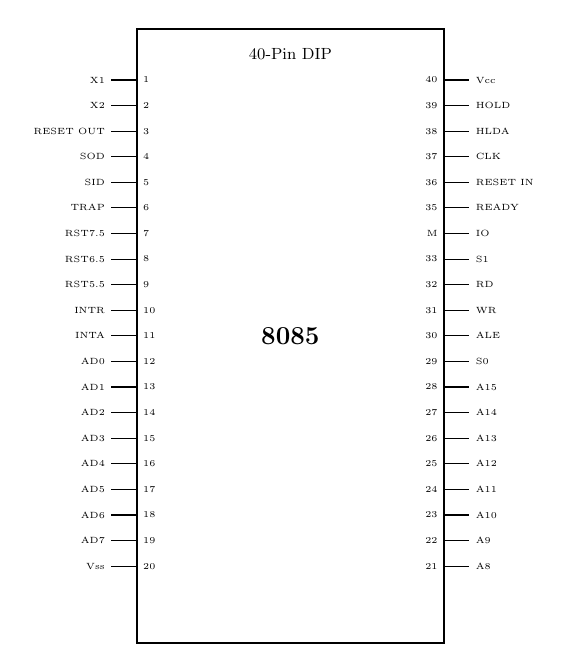
\begin{tikzpicture}[scale=0.65, transform shape]
    \draw [thick] (0,0) rectangle (6,12);
    \node at (3,6) {\Large \textbf{8085}};
    \node at (3,11.5) {\small 40-Pin DIP};
    
    % Left Pins (1-20)
    \foreach \y/\label/\pin in {
        11/X1/1, 10.5/X2/2, 10/RESET OUT/3, 9.5/SOD/4, 9/SID/5, 
        8.5/TRAP/6, 8/RST7.5/7, 7.5/RST6.5/8, 7/RST5.5/9, 6.5/INTR/10, 
        6/INTA/11, 5.5/AD0/12, 5/AD1/13, 4.5/AD2/14, 4/AD3/15, 
        3.5/AD4/16, 3/AD5/17, 2.5/AD6/18, 2/AD7/19, 1.5/Vss/20} {
        \draw (-0.5, \y) -- (0, \y);
        \node [left] at (-0.5, \y) {\tiny \label};
        \node [right] at (0, \y) {\tiny \pin};
    }
    
    % Right Pins (21-40)
    \foreach \y/\label/\pin in {
        1.5/A8/21, 2/A9/22, 2.5/A10/23, 3/A11/24, 3.5/A12/25, 
        4/A13/26, 4.5/A14/27, 5/A15/28, 5.5/S0/29, 6/ALE/30, 
        6.5/WR/31, 7/RD/32, 7.5/S1/33, 8/IO/M/34, 8.5/READY/35, 
        9/RESET IN/36, 9.5/CLK/37, 10/HLDA/38, 10.5/HOLD/39, 11/Vcc/40} {
        \draw (6, \y) -- (6.5, \y);
        \node [right] at (6.5, \y) {\tiny \label};
        \node [left] at (6, \y) {\tiny \pin};
    }
\end{tikzpicture}
\end{center}

\begin{itemize}
    \item \textbf{Address/Data}: AD0-AD7 (Multiplexed), A8-A15 (High Address).
    \item \textbf{Control \& Status}: ALE (Address Latch Enable), RD (Read), WR (Write), IO/M (Select IO or Memory), S0, S1 (Status).
    \item \textbf{Interrupts}: INTR, INTA, RST 5.5, RST 6.5, RST 7.5, TRAP.
    \item \textbf{Serial I/O}: SID (Input), SOD (Output).
    \item \textbf{DMA}: HOLD, HLDA.
    \item \textbf{Power/Clock}: Vcc (+5V), Vss (GND), X1, X2 (Crystal).
\end{itemize}
\end{solutionbox}
\begin{mnemonicbox}
``ACID-PS'' (Address-Control-Interrupt-DMA-Power-Serial)
\end{mnemonicbox}

\questionmarks{3}{a}{3}
\textbf{Explain interrupts of 8051 microcontroller.}

\begin{solutionbox}
\textbf{Answer}:

\begin{center}
\captionof{table}{8051 Interrupts}
\begin{tabulary}{\linewidth}{|l|l|l|J|}
\hline
\textbf{Interrupt} & \textbf{Vector} & \textbf{Priority} & \textbf{Source} \\ \hline
\textbf{External 0} & 0003H & 1 (Highest) & Pin INT0 (P3.2) \\ \hline
\textbf{Timer 0} & 000BH & 2 & Timer 0 overflow (TF0) \\ \hline
\textbf{External 1} & 0013H & 3 & Pin INT1 (P3.3) \\ \hline
\textbf{Timer 1} & 001BH & 4 & Timer 1 overflow (TF1) \\ \hline
\textbf{Serial} & 0023H & 5 (Lowest) & RI or TI (Serial Port) \\ \hline
\end{tabulary}
\end{center}

\textbf{Diagram:}

\begin{center}
\begin{tikzpicture}[node distance=2cm, auto]
    \node [gtu block] (cpu) {8051 CPU};
    \node [left of=cpu, node distance=3.5cm, yshift=1cm] (int0) {INT0 (P3.2)};
    \node [left of=cpu, node distance=3.5cm, yshift=0.5cm] (int1) {INT1 (P3.3)};
    \node [left of=cpu, node distance=3.5cm, yshift=0cm] (t0) {Timer 0};
    \node [left of=cpu, node distance=3.5cm, yshift=-0.5cm] (t1) {Timer 1};
    \node [left of=cpu, node distance=3.5cm, yshift=-1cm] (serial) {Serial Port};
    
    \draw [gtu arrow] (int0) -- (cpu);
    \draw [gtu arrow] (int1) -- (cpu);
    \draw [gtu arrow] (t0) -- (cpu);
    \draw [gtu arrow] (t1) -- (cpu);
    \draw [gtu arrow] (serial) -- (cpu);
\end{tikzpicture}
\end{center}
\end{solutionbox}
\begin{mnemonicbox}
``ETTES'' (External-Timer-Timer-External-Serial)
\end{mnemonicbox}

\questionmarks{3}{b}{4}
\textbf{Draw Pin diagram of 8051 microcontroller.}

\begin{solutionbox}
\textbf{Answer}:

\begin{center}
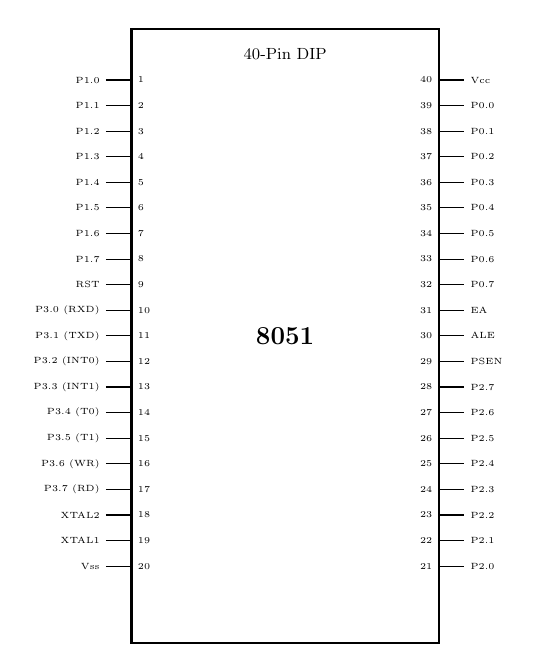
\begin{tikzpicture}[scale=0.65, transform shape]
    \draw [thick] (0,0) rectangle (6,12);
    \node at (3,6) {\Large \textbf{8051}};
    \node at (3,11.5) {\small 40-Pin DIP};
    
    % Left Pins
    \foreach \y/\label/\pin in {
        11/P1.0/1, 10.5/P1.1/2, 10/P1.2/3, 9.5/P1.3/4, 9/P1.4/5, 
        8.5/P1.5/6, 8/P1.6/7, 7.5/P1.7/8, 7/RST/9, 6.5/P3.0 (RXD)/10, 
        6/P3.1 (TXD)/11, 5.5/P3.2 (INT0)/12, 5/P3.3 (INT1)/13, 
        4.5/P3.4 (T0)/14, 4/P3.5 (T1)/15, 3.5/P3.6 (WR)/16, 
        3/P3.7 (RD)/17, 2.5/XTAL2/18, 2/XTAL1/19, 1.5/Vss/20} {
        \draw (-0.5, \y) -- (0, \y);
        \node [left] at (-0.5, \y) {\tiny \label};
        \node [right] at (0, \y) {\tiny \pin};
    }
    
    % Right Pins
    \foreach \y/\label/\pin in {
        1.5/P2.0/21, 2/P2.1/22, 2.5/P2.2/23, 3/P2.3/24, 3.5/P2.4/25, 
        4/P2.5/26, 4.5/P2.6/27, 5/P2.7/28, 5.5/PSEN/29, 6/ALE/30, 
        6.5/EA/31, 7/P0.7/32, 7.5/P0.6/33, 8/P0.5/34, 8.5/P0.4/35, 
        9/P0.3/36, 9.5/P0.2/37, 10/P0.1/38, 10.5/P0.0/39, 11/Vcc/40} {
        \draw (6, \y) -- (6.5, \y);
        \node [right] at (6.5, \y) {\tiny \label};
        \node [left] at (6, \y) {\tiny \pin};
    }
\end{tikzpicture}
\end{center}

\begin{itemize}
    \item \textbf{P0.0-P0.7}: Port 0 (Address/Data AD0-AD7).
    \item \textbf{P1.0-P1.7}: Port 1 (I/O).
    \item \textbf{P2.0-P2.7}: Port 2 (Address A8-A15).
    \item \textbf{P3.0-P3.7}: Port 3 (Special functions like RD, WR, INT).
    \item \textbf{Power}: Vcc (40), Vss (20).
    \item \textbf{Control}: RST, ALE, PSEN, EA.
\end{itemize}
\end{solutionbox}
\begin{mnemonicbox}
``PORT 0123''
\end{mnemonicbox}

\questionmarks{3}{c}{7}
\textbf{Explain Internal RAM Organization of 8051 microcontroller.}

\begin{solutionbox}
\textbf{Answer}:
Total 128 Bytes of Internal RAM (00H to 7FH).

\begin{center}
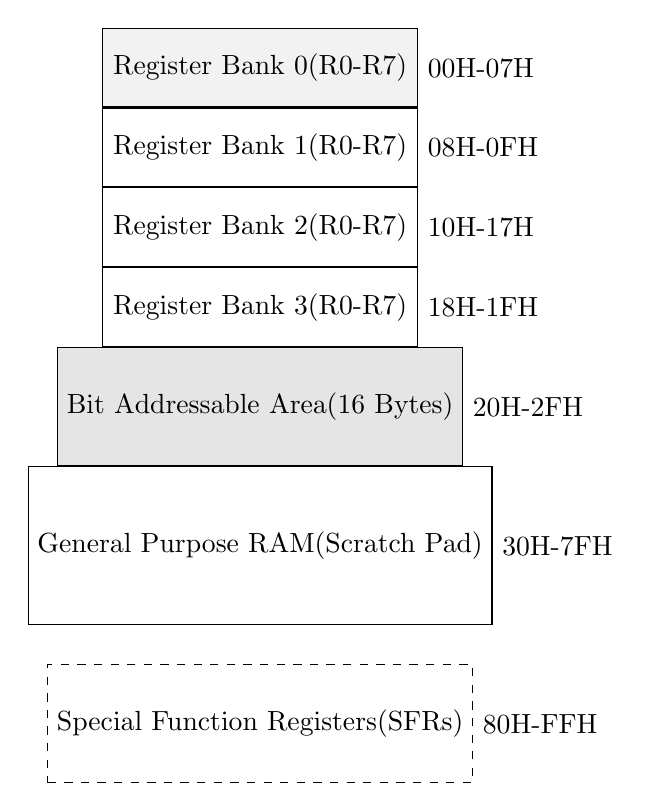
\begin{tikzpicture}[node distance=0cm, auto]
    \node [draw, minimum width=4cm, minimum height=1cm, fill=black!5] (bank0) {Register Bank 0\\(R0-R7)};
    \node [right] at (bank0.east) {00H-07H};
    
    \node [draw, minimum width=4cm, minimum height=1cm, below=of bank0] (bank1) {Register Bank 1\\(R0-R7)};
    \node [right] at (bank1.east) {08H-0FH};
    
    \node [draw, minimum width=4cm, minimum height=1cm, below=of bank1] (bank2) {Register Bank 2\\(R0-R7)};
    \node [right] at (bank2.east) {10H-17H};
    
    \node [draw, minimum width=4cm, minimum height=1cm, below=of bank2] (bank3) {Register Bank 3\\(R0-R7)};
    \node [right] at (bank3.east) {18H-1FH};
    
    \node [draw, minimum width=4cm, minimum height=1.5cm, below=of bank3, fill=black!10] (bit) {Bit Addressable Area\\(16 Bytes)};
    \node [right] at (bit.east) {20H-2FH};
    
    \node [draw, minimum width=4cm, minimum height=2cm, below=of bit] (scratch) {General Purpose RAM\\(Scratch Pad)};
    \node [right] at (scratch.east) {30H-7FH};
    
    % SFRs
    \node [draw, minimum width=4cm, minimum height=1.5cm, below=of scratch, yshift=-0.5cm, dashed] (sfr) {Special Function Registers\\(SFRs)};
    \node [right] at (sfr.east) {80H-FFH};
    
\end{tikzpicture}
\end{center}

\begin{itemize}
    \item \textbf{Register Banks (00H-1FH)}: 4 Banks of 8 registers each. Selected by RS0, RS1 bits in PSW.
    \item \textbf{Bit Addressable (20H-2FH)}: 16 bytes where each bit can be individually accessed (set/cleared).
    \item \textbf{General Purpose (30H-7FH)}: 80 bytes used for data storage and stack.
    \item \textbf{SFRs (80H-FFH)}: Mapped in upper 128 bytes (Direct Access only).
\end{itemize}
\end{solutionbox}
\begin{mnemonicbox}
``RBBS'' (Registers-Bits-Buffer-Special)
\end{mnemonicbox}

\orquestionmarks{3}{a}{3}
\textbf{List SFRs with their addresses.}

\begin{solutionbox}
\textbf{Answer}:

\begin{center}
\captionof{table}{Special Function Registers}
\begin{tabulary}{\linewidth}{|l|l|J|}
\hline
\textbf{SFR} & \textbf{Address} & \textbf{Function} \\ \hline
\textbf{P0} & 80H & Port 0 \\ \hline
\textbf{SP} & 81H & Stack Pointer \\ \hline
\textbf{DPH:DPL} & 83H:82H & Data Pointer (16-bit) \\ \hline
\textbf{PCON} & 87H & Power Control \\ \hline
\textbf{TCON} & 88H & Timer Control \\ \hline
\textbf{TMOD} & 89H & Timer Mode \\ \hline
\textbf{TL0} & 8AH & Timer 0 Low Byte \\ \hline
\textbf{TL1} & 8BH & Timer 1 Low Byte \\ \hline
\textbf{TH0} & 8CH & Timer 0 High Byte \\ \hline
\textbf{TH1} & 8DH & Timer 1 High Byte \\ \hline
\textbf{P1} & 90H & Port 1 \\ \hline
\textbf{SCON} & 98H & Serial Control \\ \hline
\textbf{SBUF} & 99H & Serial Buffer \\ \hline
\textbf{P2} & A0H & Port 2 \\ \hline
\textbf{IE} & A8H & Interrupt Enable \\ \hline
\textbf{P3} & B0H & Port 3 \\ \hline
\textbf{IP} & B8H & Interrupt Priority \\ \hline
\textbf{PSW} & D0H & Program Status Word \\ \hline
\textbf{ACC (A)} & E0H & Accumulator \\ \hline
\textbf{B} & F0H & B Register \\ \hline
\end{tabulary}
\end{center}
\end{solutionbox}
\begin{mnemonicbox}
``PDPT-SP'' (Ports-Data-Program-Timers-Serial-Prioritized)
\end{mnemonicbox}

\orquestionmarks{3}{b}{4}
\textbf{Explain Timers/Counters logic diagram of 8051 microcontroller.}

\begin{solutionbox}
\textbf{Answer}:

\textbf{Timer/Counter Logic Diagram:}

\begin{center}
\begin{tikzpicture}[auto, node distance=2.5cm]
    \node [draw, minimum width=2cm] (tl) {TLx (8-bit)};
    \node [draw, minimum width=2cm, right of=tl] (th) {THx (8-bit)};
    \draw [->] (tl) -- (th);
    \draw [->] (th) -- ++(1.5,0) node[right] {Interrupt Flag (TFx)};
    
    \node [draw, below of=tl, node distance=2cm] (control) {Control Logic};
    \draw [->] (control) -- (tl);
    
    \node [left of=control, node distance=3cm] (osc) {Oscillator $\div$ 12};
    \node [below of=osc, node distance=1.5cm] (pin) {Tx Pin (Counter)};
    
    \node [gtu block, right of=control, node distance=3cm] (mux) {C/T Mux};
    
    \draw [->] (osc) -| (mux.160);
    \draw [->] (pin) -| (mux.200);
    \draw [->] (mux) -- (control);
    
    \node [below of=mux, node distance=1cm] (gate) {GATE / TRx / INTx};
    \draw [->, dashed] (gate) -- (control);
    
\end{tikzpicture}
\end{center}

\begin{itemize}
    \item \textbf{Registers}: TLx and THx form a 16-bit register.
    \item \textbf{C/T Bit}: Selects input source. 0 = Oscillator (Timer), 1 = Tx Pin (Counter).
    \item \textbf{Control}: TRx (Run control) and GATE (External control) manage starting/stopping.
    \item \textbf{Overflow}: When count goes from FFFFH to 0000H, TFx flag is set.
\end{itemize}
\end{solutionbox}
\begin{mnemonicbox}
``TCG'' (Timer-Counter-Gate)
\end{mnemonicbox}

\orquestionmarks{3}{c}{7}
\textbf{Explain block diagram of 8051 microcontroller.}

\begin{solutionbox}
\textbf{Answer}:

\textbf{Block Diagram:}

\begin{center}
\begin{tikzpicture}[node distance=2.5cm, auto, scale=0.8, transform shape]
    \node [gtu block] (cpu) {8-Bit CPU};
    
    \node [gtu block, right of=cpu, node distance=3.5cm] (osc) {Oscillator};
    \node [gtu block, below of=cpu, node distance=2.5cm] (int) {Interrupt\\Control};
    \node [gtu block, right of=int, node distance=3.5cm] (bus) {Bus Control};
    
    \node [gtu block, left of=cpu, node distance=3.5cm] (rom) {4KB ROM};
    \node [gtu block, below of=rom, node distance=2.5cm] (ram) {128B RAM};
    
    \node [gtu block, right of=osc, node distance=3.5cm] (timers) {Timer 0\\Timer 1};
    \node [gtu block, below of=timers, node distance=2.5cm] (serial) {Serial Port\\(UART)};
    
    \node [gtu block, below of=int, node distance=3cm, minimum width=8cm] (ports) {I/O Ports (P0, P1, P2, P3)};
    
    % Connections
    \draw [gtu arrow, <->] (cpu) -- (rom);
    \draw [gtu arrow, <->] (cpu) -- (ram);
    \draw [gtu arrow] (osc) -- (cpu);
    \draw [gtu arrow] (int) -- (cpu);
    \draw [gtu arrow, <->] (cpu) -- (bus);
    
    \draw [gtu arrow, <->] (bus) -- (ports);
    \draw [gtu arrow, <->] (timers) -- (bus);
    \draw [gtu arrow, <->] (serial) -- (bus);
    
    \node [draw, dashed, fit=(cpu) (ports) (ram) (serial), inner sep=0.5cm] {};
    \node [above] at (current bounding box.north) {Internal System Bus};
\end{tikzpicture}
\end{center}

\begin{itemize}
    \item \textbf{CPU}: Brain of the system.
    \item \textbf{Memory}: 4KB ROM (Code) + 128B RAM (Data).
    \item \textbf{I/O}: 4 Ports (P0-P3) for interfacing.
    \item \textbf{Timers}: 2 16-bit timers for delay/counting.
    \item \textbf{Serial}: For communication.
    \item \textbf{Interrupts}: 5 Sources.
\end{itemize}
\end{solutionbox}
\begin{mnemonicbox}
``CAPITALS'' (CPU-Architecture-Ports-I/O-Timer-ALU-LS-Interface-Serial)
\end{mnemonicbox}

\questionmarks{4}{a}{3}
\textbf{Write an 8051 Assembly Language Program to add two bytes of data and store result in R4 register.}

\begin{solutionbox}
\textbf{Answer}:

\begin{lstlisting}[language={[x86masm]Assembler}]
MOV A, #25H       ; Load first value (25H) into Accumulator
MOV R3, #18H      ; Load second value (18H) into R3
ADD A, R3         ; Add R3 to Accumulator (A = A + R3)
MOV R4, A         ; Store result from A into R4
\end{lstlisting}

\textbf{Steps:}
\begin{enumerate}
    \item Load first operand in A.
    \item Load second operand in R3.
    \item Perform ADD operation.
    \item Move result to R4.
\end{enumerate}
\end{solutionbox}
\begin{mnemonicbox}
``LLAS'' (Load-Load-Add-Store)
\end{mnemonicbox}

\questionmarks{4}{b}{4}
\textbf{Write an 8051 Assembly Language Program to OR the contents of Port-1 and Port-2 then put the result in external RAM location 0200H.}

\begin{solutionbox}
\textbf{Answer}:

\begin{lstlisting}[language={[x86masm]Assembler}]
MOV A, P1         ; Read Port 1 into Accumulator
ORL A, P2         ; OR Accumulator with Port 2
MOV DPTR, #0200H  ; Load Data Pointer with 0200H
MOVX @DPTR, A     ; Move content of A to External RAM at 0200H
\end{lstlisting}

\textbf{Steps:}
\begin{enumerate}
    \item Read P1 to A.
    \item Logical OR with P2.
    \item Set DPTR to address.
    \item Write A to external memory using \code{MOVX}.
\end{enumerate}
\end{solutionbox}
\begin{mnemonicbox}
``PORT'' (Port-OR-Register-Transfer)
\end{mnemonicbox}

\questionmarks{4}{c}{7}
\textbf{List Addressing Modes of 8051 Microcontroller and explain them with at least one example.}

\begin{solutionbox}
\textbf{Answer}:

\begin{center}
\captionof{table}{Addressing Modes}
\begin{tabulary}{\linewidth}{|l|l|J|}
\hline
\textbf{Mode} & \textbf{Example} & \textbf{Description} \\ \hline
\textbf{Immediate} & \code{MOV A, \#25H} & Data is provided directly in the instruction (\#). \\ \hline
\textbf{Register} & \code{MOV A, R0} & Data is in one of the registers (R0-R7). \\ \hline
\textbf{Direct} & \code{MOV A, 30H} & Address of the data is given directly. \\ \hline
\textbf{Indirect} & \code{MOV A, @R0} & Address is stored in a register (@R0 or @R1). \\ \hline
\textbf{Indexed} & \code{MOVC A, @A+DPTR} & Access data from Code memory (Base + Offset). \\ \hline
\textbf{Bit} & \code{SETB P1.3} & Operation on a single bit. \\ \hline
\textbf{Relative} & \code{SJMP LABEL} & Jump to a relative address (offset). \\ \hline
\end{tabulary}
\end{center}
\end{solutionbox}
\begin{mnemonicbox}
``I'M DIRBI'' (Immediate-Register-Direct-Indirect-Relative-Bit-Indexed)
\end{mnemonicbox}

\orquestionmarks{4}{a}{3}
\textbf{Explain following instructions: (i) DJNZ (ii) POP (iii) CJNE.}

\begin{solutionbox}
\textbf{Answer}:

\begin{itemize}
    \item \textbf{DJNZ (Decrement and Jump if Not Zero)}:
    \begin{itemize}
        \item Syntax: \code{DJNZ Rn, rel}
        \item Operation: Decrement register Rn. If result is not 0, jump to relative address. Used for loops.
        \item Example: \code{DJNZ R7, LOOP}
    \end{itemize}
    
    \item \textbf{POP}:
    \begin{itemize}
        \item Syntax: \code{POP direct}
        \item Operation: Pop data from Stack to direct memory address. SP is decremented.
        \item Example: \code{POP 30H}
    \end{itemize}
    
    \item \textbf{CJNE (Compare and Jump if Not Equal)}:
    \begin{itemize}
        \item Syntax: \code{CJNE A, \#data, rel}
        \item Operation: Compare A with data. If not equal, jump. Sets Carry flag if A < data.
        \item Example: \code{CJNE A, \#25H, NEXT}
    \end{itemize}
\end{itemize}
\end{solutionbox}
\begin{mnemonicbox}
``DPC'' (Decrement-Pop-Compare)
\end{mnemonicbox}

\orquestionmarks{4}{b}{4}
\textbf{For 8051 Microcontroller with a crystal frequency of 12 MHz, generate a delay of 4ms.}

\begin{solutionbox}
\textbf{Answer}:
\textbf{Calculation:}
\begin{itemize}
    \item Crystal Freq = 12 MHz.
    \item Machine Cycle Freq = 12 MHz / 12 = 1 MHz.
    \item Time for 1 Machine Cycle = $1/1\text{MHz} = 1\mu s$.
    \item Required Delay = 4 ms = 4000 $\mu s$ = 4000 Machine Cycles.
\end{itemize}

\textbf{Program:}
\begin{lstlisting}[language={[x86masm]Assembler}]
      MOV R7, #16       ; Outer Loop: 16
DELAY1:
      MOV R6, #250      ; Inner Loop: 250
DELAY2:
      NOP               ; 1 Cycle
      NOP               ; 1 Cycle
      DJNZ R6, DELAY2   ; 2 Cycles. Total Inner = 4 * 250 = 1000
      DJNZ R7, DELAY1   ; Total = 16 * 1000 = 16000 cycles
      RET
\end{lstlisting}
\textit{Note: The above calculation in MDX (16x250x4) gives 16000 cycles = 16ms. To get 4ms, Outer loop should be 4.}

\textbf{Corrected for 4ms:}
\begin{lstlisting}[language={[x86masm]Assembler}]
      MOV R7, #08       ; Outer Loop
DELAY_LOOP:
      MOV R6, #250      ; Inner Loop (250 x 2 = 500us)
      DJNZ R6, $        ; 2 cycles per loop
      DJNZ R7, DELAY_LOOP ; 8 x 500 = 4000 us = 4ms
      RET
\end{lstlisting}
\end{solutionbox}
\begin{mnemonicbox}
``LNDD'' (Load-NOP-Decrement-Decrement)
\end{mnemonicbox}

\orquestionmarks{4}{c}{7}
\textbf{Explain any seven Logical instructions with example for 8051 Microcontroller.}

\begin{solutionbox}
\textbf{Answer}:

\begin{center}
\captionof{table}{Logical Instructions}
\begin{tabulary}{\linewidth}{|l|l|J|}
\hline
\textbf{Instruction} & \textbf{Example} & \textbf{Operation} \\ \hline
\textbf{ANL} & \code{ANL A, \#0FH} & Logical AND. Masking bits. \\ \hline
\textbf{ORL} & \code{ORL P1, \#80H} & Logical OR. Setting bits. \\ \hline
\textbf{XRL} & \code{XRL A, R0} & Logical XOR. Toggling bits. \\ \hline
\textbf{CLR} & \code{CLR A} & Clear Accumulator (A=00H). \\ \hline
\textbf{CPL} & \code{CPL A} & Complement Accumulator (Invert bits). \\ \hline
\textbf{RL} & \code{RL A} & Rotate Left (circular shift). \\ \hline
\textbf{RR} & \code{RR A} & Rotate Right (circular shift). \\ \hline
\end{tabulary}
\end{center}
\end{solutionbox}
\begin{mnemonicbox}
``A-OX-CCR'' (AND-OR-XOR-Clear-Complement-Rotate)
\end{mnemonicbox}

\questionmarks{5}{a}{3}
\textbf{List Applications of microcontroller in various fields.}

\begin{solutionbox}
\textbf{Answer}:

\begin{itemize}
    \item \textbf{Industrial}: Motor control, Automation, PLCs.
    \item \textbf{Medical}: Patient monitoring, X-ray machines.
    \item \textbf{Consumer}: Washing machines, Microwave ovens, Toys.
    \item \textbf{Automotive}: ECU, ABS, Airbags.
    \item \textbf{Communication}: Modems, Routers, Mobile phones.
    \item \textbf{Security}: CCTV, Biometric systems.
\end{itemize}
\end{solutionbox}
\begin{mnemonicbox}
``I-MACS'' (Industrial-Medical-Automotive-Consumer-Security)
\end{mnemonicbox}

\questionmarks{5}{b}{4}
\textbf{Interface Push button Switch and LED with 8051 microcontroller.}

\begin{solutionbox}
\textbf{Answer}:

\textbf{Circuit Diagram:}

\begin{center}
\begin{tikzpicture}[auto, node distance=2.5cm]
    \node [gtu block, minimum height=3cm] (mcu) {8051};
    
    % Switch
    \node [left of=mcu, yshift=1cm, node distance=2cm] (sw_pin) {};
    \draw (mcu.west |- sw_pin) -- ++(-1,0) node[circ] (node1) {} -- ++(0, 0.5) node[above] {Vcc} node[midway, right] {10k};
    \draw (node1) -- ++(0,-0.5) -- ++(-0.5,0) node[draw, rectangle] (sw) {SW} -- ++(0,-0.5) node[ground] {};
    \node [right] at (mcu.west |- sw_pin) {P1.0};
    
    % LED
    \node [left of=mcu, yshift=-1cm, node distance=2cm] (led_pin) {};
    \draw (mcu.west |- led_pin) -- ++(-1,0) to[R, l=330$\Omega$] ++(-1.5,0) node[circ] {} to[nativeLED] ++(-1,0) node[ground] {};
    \node [right] at (mcu.west |- led_pin) {P1.7};
    
\end{tikzpicture}
\end{center}

\textbf{Program:}
\begin{lstlisting}[language={[x86masm]Assembler}]
AGAIN:
    JB P1.0, LED_OFF  ; If P1.0 is High (Not pressed), Jump
    SETB P1.7         ; If Low (Pressed), Turn ON LED
    SJMP AGAIN
LED_OFF:
    CLR P1.7          ; Turn OFF LED
    SJMP AGAIN
\end{lstlisting}
\end{solutionbox}
\begin{mnemonicbox}
``PLIC'' (Push-LED-Input-Control)
\end{mnemonicbox}

\questionmarks{5}{c}{7}
\textbf{Interface LCD with microcontroller and write a program to display "HELLO".}

\begin{solutionbox}
\textbf{Answer}:

\textbf{Circuit Diagram:}

\begin{center}
\begin{tikzpicture}[auto, node distance=3cm]
    \node [gtu block, minimum height=3cm] (mcu) {8051};
    \node [gtu block, right of=mcu, node distance=5cm, minimum height=3cm] (lcd) {16x2 LCD};
    
    \draw [->, thick] (mcu.east) -- (lcd.west) node[midway, above] {Data (P2.0-P2.7)};
    
    \draw [->] ($(mcu.east)+(0,-1)$) -- ($(lcd.west)+(0,-1)$) node[midway, above] {Ctrl (P3.0-P3.2)};
    \node [right] at ($(lcd.west)+(0,-1.3)$) {RS, RW, E};
\end{tikzpicture}
\end{center}

\textbf{Program:}
\begin{lstlisting}[language={[x86masm]Assembler}]
    MOV A, #38H       ; Init LCD 2 lines, 5x7
    ACALL CMD
    MOV A, #0EH       ; Display ON, Cursor ON
    ACALL CMD
    MOV A, #'H'       ; Data 'H'
    ACALL DISP
    MOV A, #'E'
    ACALL DISP
    MOV A, #'L'
    ACALL DISP
    MOV A, #'L'
    ACALL DISP
    MOV A, #'O'
    ACALL DISP
    SJMP $
    
CMD: MOV P2, A        ; Send Command
     CLR P3.0         ; RS=0
     CLR P3.1         ; RW=0
     SETB P3.2        ; E=1
     ACALL DELAY
     CLR P3.2         ; E=0
     RET
     
DISP: MOV P2, A       ; Send Data
      SETB P3.0       ; RS=1
      CLR P3.1        ; RW=0
      SETB P3.2       ; E=1
      ACALL DELAY
      CLR P3.2
      RET
\end{lstlisting}
\end{solutionbox}
\begin{mnemonicbox}
``DICE'' (Data-Instruction-Control-Enable)
\end{mnemonicbox}

\orquestionmarks{5}{a}{3}
\textbf{Draw Interfacing of LM35 with 8051 microcontroller.}

\begin{solutionbox}
\textbf{Answer}:

\begin{center}
\begin{tikzpicture}[auto, node distance=2.5cm]
    \node [gtu block] (mcu) {8051};
    \node [gtu block, left of=mcu, node distance=4cm] (adc) {ADC0804};
    \node [gtu block, left of=adc, node distance=3cm] (lm35) {LM35};
    
    \draw [->] (lm35) -- (adc) node[midway, above] {Analog V};
    \draw [->, thick] (adc) -- (mcu) node[midway, above] {Data (P0)};
    \draw [<->, dashed] (adc) -- (mcu) node[midway, below] {Ctrl (P1)};
    
    \node [below of=lm35] {Temp Sensor};
    \node [below of=adc] {A/D Converter};
\end{tikzpicture}
\end{center}
\end{solutionbox}
\begin{mnemonicbox}
``TAC'' (Temperature-Analog-Convert)
\end{mnemonicbox}

\orquestionmarks{5}{b}{4}
\textbf{Interface Stepper motor with 8051 microcontroller.}

\begin{solutionbox}
\textbf{Answer}:

\textbf{Circuit:}

\begin{center}
\begin{tikzpicture}[auto, node distance=3cm]
    \node [gtu block] (mcu) {8051 (P1)};
    \node [gtu block, right of=mcu] (driver) {ULN2003};
    \node [gtu block, right of=driver] (motor) {Stepper\\Motor};
    
    \draw [->, thick] (mcu) -- (driver) node[midway, above] {4 Lines};
    \draw [->, thick] (driver) -- (motor) node[midway, above] {Coils};
\end{tikzpicture}
\end{center}

\textbf{Logic:}
\begin{itemize}
    \item Send sequence: 0x08, 0x0C, 0x04, 0x06, 0x02, 0x03, 0x01, 0x09.
    \item Delay between steps determines speed.
\end{itemize}
\end{solutionbox}
\begin{mnemonicbox}
``PDCS'' (Port-Driver-Current-Sequence)
\end{mnemonicbox}

\orquestionmarks{5}{c}{7}
\textbf{Interface ADC0804 with 8051 microcontroller.}

\begin{solutionbox}
\textbf{Answer}:

\textbf{Interfacing:}

\begin{center}
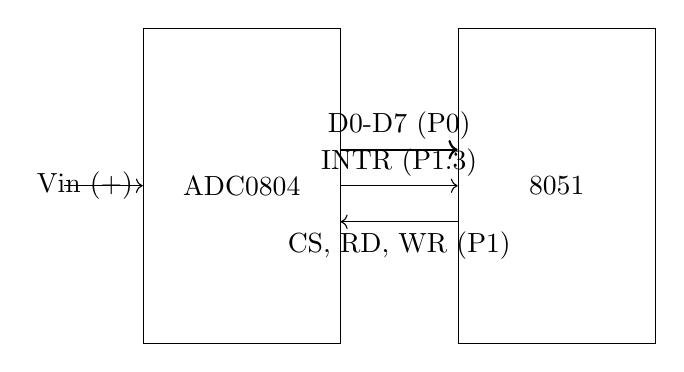
\begin{tikzpicture}[auto, node distance=4cm]
    \node [draw, minimum height=4cm, minimum width=2.5cm] (adc) {ADC0804};
    \node [draw, minimum height=4cm, minimum width=2.5cm, right of=adc] (mcu) {8051};
    
    \draw [->, thick] (adc.20) -- (mcu.160) node[midway, above] {D0-D7 (P0)};
    \draw [<-] (adc.-20) -- (mcu.-160) node[midway, below] {CS, RD, WR (P1)};
    \draw [->] (adc.east) -- (mcu.west) node[midway, above] {INTR (P1.3)};
    
    \node [left] at (adc.west) {Vin (+)};
    \draw [<-] (adc.west) -- ++(-1,0); 
\end{tikzpicture}
\end{center}

\textbf{Control Signals:}
\begin{enumerate}
    \item \textbf{CS=0}: Select Chip.
    \item \textbf{WR=0 then 1}: Start Conversion.
    \item \textbf{Wait for INTR=0}: Conversion Complete.
    \item \textbf{RD=0}: Read Data.
\end{enumerate}
\end{solutionbox}
\begin{mnemonicbox}
``CRIW'' (Control-Read-Interrupt-Write)
\end{mnemonicbox}

\end{document}
